\section{Recursive CTEs}
Recursive CTEs iteratively traverse hierarchical data of arbitrary length, and similarly to algorithms contain a base case (stop condition) and its recursive step. The number of times to iterate does not have to be constant.

\begin{lstlisting}[language=SQL]
with recursive r (i) as (
	select 1
	-- non-recursive term
	union all
	-- recursive term
	select i + 1
	from r
	where i < 5)
select * from r;
\end{lstlisting}

Recursive expressions can be used to manipulate data in a hierarchical structure. The non-recursive part defines the base case with eventual deterministic checks, while the recursive table traverses the tree upwards applying conditions.

Every recursive query can be defined by a simple evaluation algorithm: 
\begin{lstlisting}[language=Matlab]
workingTable = evaluateNonRecursive()
output workingTable
while workingTable is not empty
	workingTable = evaluateRecursive(workingTable)
	output workingTable
\end{lstlisting}

It is important to notice that the working table gets fully replaced at every iteration of the second part.

It is also possible to increment counters within RCTEs, and create trees. To avoid infinite loops in cyclic structures, using \texttt{UNION} instead of \texttt{UNION ALL} allows to remove duplicates and checking before writing a new value.

To avoid loops within graphs, a NOT EXISTS condition can be added to check whether a node has already been discovered. 

Best practices to deal with graph-like data involve knowing its cardinality, to be aware of the maximum distance, yet most problems are Turing complete.

Postgres only allows one mention of the recursive relation in the recursive subquery.

\section{Window functions}
Window functions are versatile tools to implement time series analysis, percentiles and cumulative sums. 

A window function can be seen as a special case of aggregate, evaluated after every clause but ORDER BY, but opposite to aggregation they do not change the result: only additional columns are computed.

The term window describes the set of rows on which the window operates, returning values from it. 

Example (from Postgres documentation):
\begin{lstlisting}
select product_name, 
	price, 
	group_name, 
	avg(price) over (
			partition by group_name
			)
from products
	inner join product_groups
	using (group_id);
\end{lstlisting}
The previous query returns the product name, the price, product group name, along with the average prices of each product group.

AVG works as window function, operating on the subset of rows specified by OVER. 

PARTITION BY distributes the rows of the result set into groups, each one of them subject to AVG, returning the average price.

Calculations on window functions are always performed on the result set after the other clauses but ORDER BY.

General window functions syntax:
\begin{lstlisting}
window_function(arg1, arg2,..) OVER (
	[PARTITION BY partition_expression]
	[ORDER BY sort_expression [ASC | DESC] [NULLS {FIRST | LAST }]
	[frame_clause])
\end{lstlisting}

To summarize:
\begin{itemize}
	\item The window function is an aggregate function, such as SUM or AVG;
	\item The (optional) partitioning clause divides the rows into multiple groups;
	\item The ordering clause specifies the order of internal rows;
	\item The framing clause defines a subset of rows in the current partition to which the window function is applied.
\end{itemize}

Multiple window functions can also be applied in the same query. Some other examples which ignore framing are:
\begin{itemize}
	\item Ranking:
	\begin{itemize}
		\item \texttt{rank()} and \texttt{dense\_rank()}, returning the rank of the current row with or without gaps;
		\item \texttt{row\_number()};
		\item\texttt{ ntile(n)}, distributing data over buckets;
	\end{itemize}
	\item Distribution:
	\begin{itemize}
		\item \texttt{percent\_rank()} and \texttt{cume\_dist()}, returning the relative rank of the current row or peer group (rows with equal partitioning);
	\end{itemize}
	\item Navigation:
	\begin{itemize}
		\item \texttt{lag(expr, offset, default)} and \texttt{lead(expr, offset, default)} evaluate the expression respectively on preceding and following row.
	\end{itemize}
\end{itemize}

Framing can follow only a few specifications, not too complex:
\begin{itemize}
	\item \texttt{current row};
	\item \texttt{unbounded preceding} or \texttt{unbounded following}, first and last row in the partition;
	\item \texttt{range between unbounded preceding and current row}, default frame with order specified;
	\item \texttt{range between unbounded preceding and unbounded following}, default frame with order unspecified;
	\item \texttt{aggregates()}, computing aggregates over all tuples in current frame;
	\item \texttt{first\_value()}, \texttt{last\_value()}, \texttt{nth\_value()}, evaluating an expression on determined rows of the frame.
\end{itemize}

\subsection{Segment trees}
Segment trees are an useful data structure for efficient evaluation, used for storing information related to intervals (segments).

Querying a static segment tree allows knowing which of the stored segments contains a given element, using logarithmic time operations.

The set of existing values gets divided into possible interval endpoints, sorted from left to right. All leaves in the tree correspond to the elementary intervals induced by endpoints, while internal nodes are the union of two intervals. 

Any interval is stored in the canonical set for at most two nodes at the same depth, therefore the required storage is $O(n \log n)$ with $n$ intervals.

Space for leaves is linear, and aggregated functions can be calculated on intervals very quickly. 

Segment trees are useful for window functions, since intervals can be seen as windows, either static or sliding. For each call of a window function, a new segment tree gets built: the time for construction is just linear, since ordering is already performed by the ORDER BY clause.

\subsection{Other aggregates}
Newer version of Postgres allow calculation of more complex statistical aggregates, such as standard deviation, correlation and linear regression.

Mode and percentiles are also supported, yet they require materialization and sorting therefore they need a special syntax and the clause \texttt{within group}.

\subsubsection{Grouping sets}
A grouping set is a set of columns by which data is grouped, for instance using aggregates. They can be unified using UNION ALL.

Since uniting requires all sets to have the same number of columns, eventual inconsistencies must be filled with NULL: this is both lengthy and nonperforming (linear scans).

GROUPING SETS, a GROUP BY option, allows to define multiple grouping sets in the same query. It is possible to group by one or multiple columns, or even nothing. Missing values are automatically filled with NULL.

ROLLUP calculates all the grouping possibilities ($2^n$) and applies them. 

\section{Database clusters}
Storing a large quantity of data on a single machine can have limitations: performance is restricted to hardware, and in case of failure transactions get lost. 

Using multiple machines is therefore a valid solution to handle databases: clusters are transparent and present themselves as a single system, still maintaining consistency between nodes. 

\subsection{ACID vs BASE}
ACID and BASE are two standards to describe the properties of databases. One could be defined as the opposite of the other, because their usage is distinct between relational models and NoSQL.

\begin{itemize}
	\item Atomic: all operations in a transaction must either succeed or be reverted;
	\item Consistent: each transaction is always propagated to all nodes;
	\item Isolated: transactions do not contend with one another;
	\item Durable: results are permanent, even with failures.
\end{itemize}

\begin{itemize}
	\item Basically Available: ensures an operating cluster yet not all data might be immediately accessible after a failure;
	\item Soft state: data needs to be periodically refreshed, it does not have a permanent state;
	\item Eventual consistency: consistency is not achieved all the time, but will be reached at some point after a number of updates.
\end{itemize}

Both models have advantages and disadvantages, but generally BASE properties are much looser and less strict than ACID. 

BASE does not provide a consistent view of the data, which can lead to confusion and cannot be used for critical systems, therefore it should only be used when performance is more important than ACID guarantees.

\subsection{CAP theorem}
The CAP theorem states that is impossible for a distributed database to simultaneously achieve more than two of the following guarantees:
\begin{enumerate}
	\item Consistency (every read receives either the most recent write or an error);
	\item Availability (every request receives a response);
	\item Partition tolerance (system operating even with dropped messages or delays).
\end{enumerate}
Partition tolerance is not really an option: some systems cannot be partitioned (servers with no replication), and for a distributed system not guaranteeing partition tolerance would imply to never drop messages and never have a dying node.

The probability of any node to fail increases exponentially as the number of total nodes increase.

When a network partition failure happens, therefore, the choice has to be between canceling the operation decreasing availability or proceed propagating it risking consistency.

If a system chooses to provide consistency, it will preserve atomic reads but refuse to respond to some requests.

If, on the other hand, availability is chosen, the system will respond to all requests, potentially returning outdated information and accepting conflicting writes. 

\subsection{Transaction handling}
In distributed systems, transactions should be atomic. This means there are two options for ending one:
\begin{itemize}
	\item Commit, the transaction was successful and it can become persistent and visible to all nodes;
	\item Abort, the transaction failed or violates a constraint, therefore the system needs to be reverted to its previous state.
\end{itemize}
Since node crashes in a distributed system are independent, the protocol needs to be extended to ensure atomicity of transactions: a valid method is two-phase locking (2PL). 

It is characterized by the presence of a coordinator node which allows $n$ agents of a system $A_1, A_2, \dots, A_n$ to either all persist the changes of $T$ or all discard them.

This is a commitment protocol that coordinates all processes participating in a distributed atomic transaction, achieving its purpose using logging of the states to aid recovery procedures.

The two phases of the protocol in a normal execution are:
\begin{itemize}
	\item Commit-request phase, in which a coordinator process attempts to prepare all the processes participating to the transaction to take the necessary steps and vote whether the operation can be committed;
	\item Commit phase, based on the votes, whose result gets communicated to the participants and the needed actions to commit or abort are taken.
\end{itemize}

Message flow in 2PL with 4 agents:
\begin{figure}[h]
	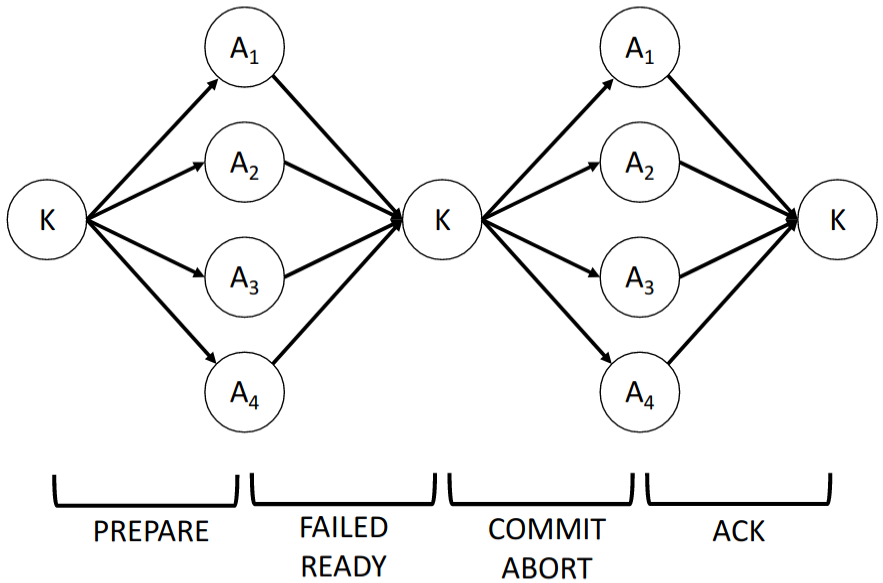
\includegraphics[scale=0.4]{2pc.png}
	\centering
\end{figure}

Issues of this method include the crash of nodes (both coordinator and agent) or potential lost messages.

\subsection{Replication}
Replication is a technique consisting in keeping a copy of the dataset in each machine. Redundant resources improve query throughput, can accommodate node failures and solve locality issues.

Access to a replicated entity is typically uniform with access to a single non-replicated entity, and copying should be transparent to external users. 

Systems can also use a master-slave scheme, predominant in high availability clusters, where a single node is designated to process all requests. 

\subsubsection{Horizontal partitioning}
Horizontal sharding involves every machine having only a chunk of the dataset. Query runtimes are improved, yet communication between shards should be minimized, due to network throughput.

Performance, in fact, relies heavily on the used interconnect, but allows nodes to have much less occupied memory so that dataset eveb bigger than the capacity of the machine can be accommodated.

Optimization of queries imply processing clauses separately, locally on each node, and aggregating results later so that the least amount of data is sent.

\subsubsection{Shard allocation}
Shards can be allocated to the cluster machines in different ways:
\begin{itemize}
	\item Every machine receives one shard;
	\item Every machine receives multiple shards.
\end{itemize}
Having more shards than machines results in better skew handling: they can take advantage of the resources available on nodes, increasing performance.

Also, there is no guarantee that the chosen hashing is uniform, and when values in between different shards are queried, it is likely that they are not all on the same machine.

Replication and sharding can be applied together, combining the benefits of both, but this leads to an increased resource consumption.
\begin{figure}[h]
	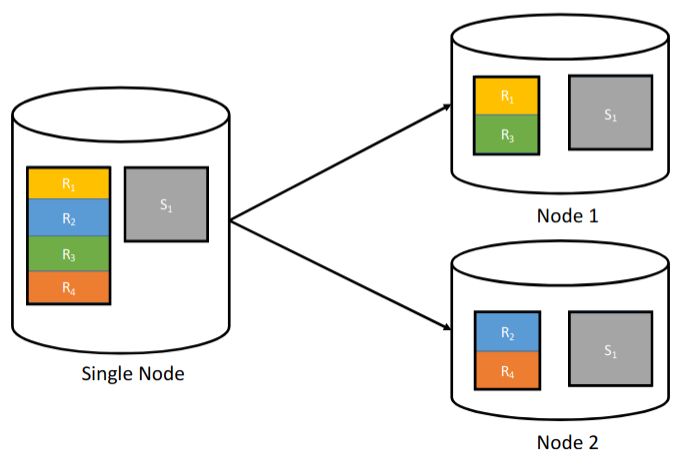
\includegraphics[scale=0.5]{replication_sharding.png}
	\centering
\end{figure}

\subsection{Joins}
Joins in a distributed system are not different than local ones in presence of a replicated environment, yet can become complicated when data is sharded across multiple machines. 

\subsubsection{Co-located joins}
A co-located join is the most efficient way to join two large distributed tables: every table has a common distributed column and is sharded across machines in the same way.

All rows with the same column, therefore, are always on the same machine, even across different tables, so that relational operations can be performed within the groups.

The joins can be executed in parallel locally on the workers, returning results to the coordinator node.

\subsubsection{Distributed joins}
A distributed join involves data which is sharded across several nodes.

Data is usually filtered as much as possible before being sent, but data movement is still necessary for joining: all nodes send their part of the table to a single one for it to run operations.

This join is only performing when the number of rows is small, otherwise the node doing the join will be overwhelmed by the dataset size and unable to parallelize.

\subsubsection{Broadcast joins}
A broadcast join is applicable when only one side of the join requires a small set of rows (small table or very selective filter).

The side of the join with the small set is sent to every node in the cluster, then joined locally with the large table on the other side of the join.

\subsubsection{Considerations}
All the previous methods still needs to consider size of the tables and bandwidth: some operations might be faster reading the data from remote machines rather than on local disks, since cache size is limited.

In this case, data can be shared to multiple nodes, each of them storing a partition of the table and computing local results which are then aggregated.

Postgres supports read replicas, kept in sync for consistent reads: each application can send data either to the master or the slaves, and the master itself can also trigger replication.

However, it is not natively a distributed database: its alternative Greenplum (still based on Postgres) allows data distribution and partitioning, both of data and schema. 

Distributed and partitioning schemes can be specified creating a table, adding DISTRIBUTED BY to define how data is spread, or PARTITION BY for partitioning within a segment.

Distributions may be round-robin (as evenly as possible, non-deterministic), or hashed (rows dispersed according to a hash function).

\begin{figure}[h]
	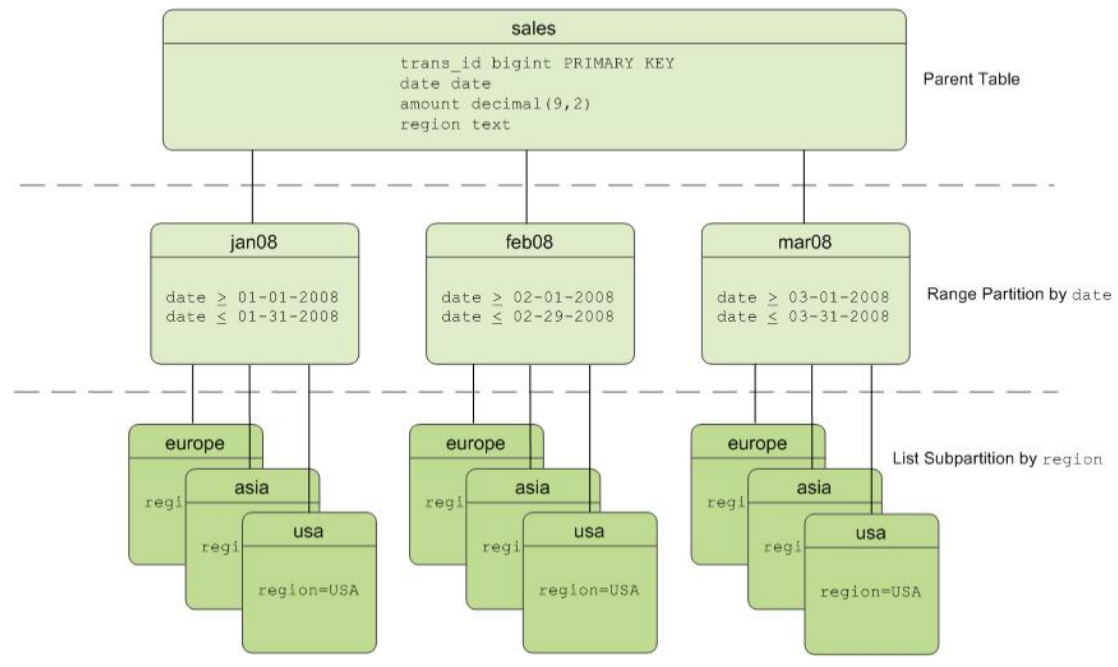
\includegraphics[scale=0.38]{greenplum.png}
	\centering
\end{figure}

MemSQL is another distributed database system based on SQL, which also allow replication, distributed and co-located joins.

A MemSQL cluster consists of aggregator and leaf nodes: aggregators handle metadata, monitoring and results of queries, while leaves act as storage layer and execute queries. 

By default, MemSQL shards tables by their primary key, while manual sharding needs to be specified.

Distributed systems overall have more resources, but their synchronization might be expensive.

\section{Autonomous database systems}
Autonomous database systems are designed to remove the burden of managing DBMS from humans, focusing on physical database design and configuration/query tuning. The first attempts to program self-adaptive systems were in the 1970s, and have now evolved to learned components. 

Indexing has been replacing with a neural network which predicts the location of a key, and transaction are scheduled through the machines by learned scheduling with unsupervised clustering. The most promising innovation is learned planning, deep learning algorithms which help running the query planner, estimating the best execution order of the operations. 

A self driving DBMS is therefore a system that configures, manages and optimizes itself for the target database and its workload, using an objective function (throughput, latency) and some constraints. The two components of this are an agent (the one who makes decisions and learns over time) and an environment, the subject of the actions. Environments have a state used as feedback for the agent. This system can help exploring unknown configurations (and their consequences) and generalizing over applications or hardware.

\subsection{State modeling}
State modeling concerns the representation of the environment state, and has to be performed in an accurate way. The model is stochastic, non stationary and episodic (there is a fixed endpoint), and it can be represented with a Markov decision process model. The entire history of the DBMS is encoded in a state vector: its contents, design, workload and resources.

The table state contains number of tuples, attributes, cardinality and other values which altogether contribute to the choice of specific implementations (for instance indexes), but changes are constrained since the number of dimensions of the feature vectors always has to be the same. The content is approximated through a state vector, therefore there is no precise information regarding how the actual table looks like. 

The knob configuration state depends on the machine, and is not really scalable. Not every configuration is applicable to servers, but one potential solution is to store hardware resources according to their percentages in respect of the available amount. 

Feature vectors can be reduced (PCA), exacerbating instability, and hierarchical models help isolating components to reduce the propagation of changes. 

Acquisition of data is done through targeted experiments while the system is running in production, training the model with end-to-end benchmarks of sample workloads. Instead of running the full system, micro-benchmarks can be run on a subset of components. This method is more effective and requires less iteration to converge. 

To avoid slowing down the entire system, training is performed on replicas (master-slave architecture) having an agent recognize the resources and eventually propagating the best changes to the master. The application server primarily communicates with the master through reads and writes, and obtaining a complete view of all the operation is sometimes hard since not everything is sent to the replicas (failed queries, for instance). 

An alternative is imitation learning: the model observes a tuned DBMS and tries to replicate those decisions. The state of the database still needs to be captured to extrapolate why changes have been applied, and training data will be sparse or noisy.

\subsection{Reward observation}
Rewards are classified as short-term and long-term, the latter more problematic since it is difficult to predict the workload trends. Transient hardware problems are hard to detect and could mask the true reward of an action, so current benchmarks have to be compared with historical data to reconsider recent events. 

Many systems concern both OLTP and OLAP workloads, and changes in the objective functions may have a negative impact on either. Generally multiple policies define preference of one over th other in mixed environments. 

Other common problems regard action selection policies, transparency and human interaction. 
